\chapter{Experimental Evaluation}
\label{cha:results}

In this chapter, all the finding will be presented during the testing phase. Three games were tested: the Hearts Game, the Maze Game, and the Puzzle Game. During these testings data was gathered from gameplay sessions and post-interviews with children between the age of six and seven years old.

These games were designed to help children with specific learning disabilities like dyslexia, dyscalculia, and other challenges. The tests were only made with children that were not diagnosed with LDs.

The aim is to understand how well these games engaged the children, supported their learning, and addressed their difficulties.

\newpage

\section{Testing process and limitations}

For these studies, tests were conductucted regarding three out of the five minigames developed in this project.
With the help of the teachers, Salomé Alves and Ana Cardoso, from the school EB1/JI da Portela. This school has multiple students from the first to fourth grade, having children between the ages of six to ten.
The testing scenario was done in the Class 1A, correspondant to the first graders.
The teacher played an essential role in coordinating the testing sessions, ensuring the children understood the instructions, and providing support throughout the process.

Originally, the goal of these tests were to test specifically with children who have LDs. Unfortunately, this was not possible. Due to several factors, the orienting team of the project was not able to reach a large enough group of children with LDs. Some of the challenges include the limited access to specialized schools and restrictions to obtaining parental consent for participation. We decided to carry out a test scenario with a broader group of children.

Despite the children in the current study not necessarily having LDs, it still provides us with valuable insights on the developed project. Like mentioned before, all the games share similar design, interactions, narratives and levels. The feedback received from the children, helped identify universal issues also affect children with LDs, such as the need for clearer instructions, and the effectiveness of visual aspects of the game. This feedback are directly applicable to refining all five games.

Moreover, many of the challenges observed, like motor coordination problems and the difficulty some children had in focusing, are issues that are also commonly faced by children with LDs. With this in mind, the problems identified and the corresponding improvements suggested are relevant to the target group in mind in the beginning.

The two games that were not tested still benefit from the critiques raised through the three tested games, given their similar structures and shared design.

\newpage
\section{Results}

In this section, it is intended to go in depth in the tests performed in the classrooom. It's important to notice that, for each game, data was gathered in two batches. The first one was the observing of the children during the \textbf{gameplays} and even small conversation while the children is playing the game. The second and last part was a small post interview to gather \textbf{feedback} from the children such as pros, cons and some observations the children might have.

The informations retrieved were the following.

\paragraph{Gameplay}
\begin{itemize}
    \item Difficulties
    \item Game Score
    \item Quality
    \item Is the game easy?
    \item Comments
    \item Socializing
    \item Observations
\end{itemize}

\paragraph{Feedback}
\begin{itemize}
    \item Did you like the game?
    \item Are levels hard?
    \item Did you like all the levels?
    \item Did you like the stories?
    \item Was it hard to understand what to do?
    \item Did you learn anything?
    \item Could it be more fun? How?
    \item Would you like to play it everyday?
    \item Do you want to play it with friends?
\end{itemize}


\subsection{Maze Game Results}
The game had players move Mr. Pig through a maze, collecting items before finding the exit. As players moved to higher levels, the mazes got bigger and more complicated.

Many kids found the controls difficult. Some had trouble using the mouse, especially on larger levels. Others breezed through the early stages but struggled with the harder ones later on. This shows that while some levels were too easy for certain kids, others were quite challenging. Comments like “move, pig” and “the little pig doesn’t want to go” were common, highlighting how character movement was tricky for some. It suggests that using the mouse was a major obstacle for many of them.

Despite some difficulties, most children said they enjoyed the game. Many of them were enthusiastic, with responses like “sim, jogaria todos os dias” being common. However, there were also some suggestions for improvement, such as making Mr. Pig move faster or simplifying the controls.

Overall, the Maze Game was engaging for the kids, though it highlighted issues with motor coordination, especially for those using a mouse. This shows how important it is to simplify controls for children who have motor skill challenges. The narrative—about Mr. Pig cleaning up the garbage—seemed to resonate well with the children, which kept them motivated despite the control issues.

With these issues in mind. The game's control, that was previously done just with mouse drag and dropping, was changed allowing for the users to play with the 'ASWD' or arrow keys. This was done so that, if movement with the mouse is tricky the user can use other options.

\newpage
\subsection{Puzzle Game Results}

The Puzzle Game featured ecology-themed puzzles with three levels of difficulty to choose from. The players had to place pieces into a puzzle using a tray.

The children’s performance varied widely. Some completed the puzzles quickly, while others needed some assistance. There were also some that showed a lot of enthusiasm, mentioning that he was ''“very good at puzzles''. However, some children, didn’t notice the reference images provided, which might have made solving the puzzles easier for them.

The Puzzle Game seemed to be well received, but it was clear that some children needed more help noticing important visual cues, like the reference image. For this, the reference image was made more obvious with the help of a frame around it, making it clearerer to the users and improving the experience. The figure \ref{fig:puzzleRefImage} details the new reference image.

\begin{figure}[!h]
    \centering
    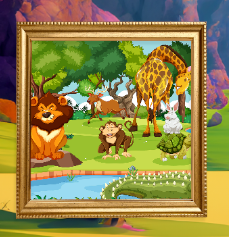
\includegraphics[width=0.3\linewidth]{Chapters/game_changes/puzzle-game-frame.png}
    \caption{Reference Image Frame}
    \label{fig:puzzleRefImage}
\end{figure}

Overall, the positive comments and the children’s eagerness to play again show that puzzles can be an effective way to develop problem-solving skills.

\subsection{Hearts Game Results}

The Hearts Game was about collecting items and following a story as the levels got harder.

Some children had trouble concentrating and needed help, especially on the difficult levels. One child needed assistance on the third level, which she found tough. A few kids struggled with controlling the game, particularly when using the mouse.

Feedback was mixed. Two enjoyed the game and said they’d like to play it again. Others found it too hard and weren’t eager to replay. One mentioned it could be more enjoyable but didn’t offer specific suggestions. The story didn’t engage everyone; responses varied when asked, “Did you like the stories?”.

The game highlighted challenges with control and understanding. The difficulty of some levels and unclear instructions made it less fun for some children. Simplifying the controls and offering more guidance on harder levels could make the game better. However, the positive feedback from others suggests the story aspect could work well with some improvements.

\newpage
\subsection{Discussion}

With the results in mind we can see both success and improvement areas. The children displayed a lot of enthusiasm, some wanting to play them regularly. The tests provided us with real feedback such as recurring issues with the control in the Maze Game for instance, that was quickly fixed after, simplifying the control schemes. Also the issue with the visual cues provided in the Puzzle Game not being well accessible by some players that was also fixed later on.


The feedback highlighted the importance of engaging content that matches the children’s interests, such as ecology and familiar characters. The games did well in capturing their attention and gave the valuable insights into how different game mechanics impact engagement and learning for kids with learning disabilities.

One common thing that happened sometimes was that the children sometimes skipped the games stories and instructions and sometimes had to come back and read it in order to know how to play the games. To simplify this, the reading out loud feature was created and set to read each game's story before starting it, along with a new button that allows for the enabling/disabiling the reading out loud (fig. \ref{fig:readInstructionsButton}).

\begin{figure}[!h]
    \centering
    
\includegraphics[width=0.1\linewidth]{Chapters/game_changes/read-sound-icon.png}
    \caption{Read Instructions Button}
    \label{fig:readInstructionsButton}
\end{figure}

Overall, the enthusiasm shown by many of the children indicates that educational games have great potential to support learning when they are designed with their needs in mind.

% Going forward, some things that would totally increase the quality of the games, would be the access for multiple languages. Right now, the games are tailored to a specific group of children and, the ability to add new levels is quite simple being a developer. This is due to the simplicity of the design of the software. Despite this, because these games are to be used in schools and medical centres, the end game is to let the teachers or doctors or anyone assisting the gameplay to children to be able to edit and create a completely different narrative for each children. What can be proposed is a new area to the main menu, where the tutor can manage each game and customize the gameplay. This could include changing the story, icons, and adding or removing levels.